\section{Generación de los \glspl{BT}}
\label{sec:GeneracionBTs}

% Una vez se lanza el proceso de Python, se recogen los argumentos de la ejecución mediante el módulo ``sys''.
En un principio se planteó la generación de los \glspl{BT} de forma directa, en la que se le pasaba el prompt del usuario a un modelo local y éste generaba un \gls{BT} en el formato JSON especificado en el apéndice \ref{appendix:Schema}.
Este planteamiento se realizaba mediante el módulo de Python ``guidance'', el cual permite forzar un formato de salida a un modelo de \gls{Ollama}.
Para este caso se probaron diferentes modelos, todos probados bajo el mismo escenario y con la temperatura en 0.0:
\begin{itemize}
    \item \texttt{Prompt}: \gls{npc} that, constantly, select a random point from the map, goes to the point and waits a time.
    \item \texttt{Acciones disponibles}: ChooseRandomPoint, MoveTo, WaitTime, RotateToFaceBBEntry.
    \item \texttt{Variables de la \gls{BB}}: Point (Vector3)
\end{itemize}

Se buscó una tarea sencilla para establecer un baseline de los modelos.
Los modelos probados para este planteamiento, con sus parámetros, su tiempo de ejecución y su resultado se pueden ver en la tabla \ref{tab:modelos-guidance}:

\begin{longtblr}[
    caption = {Modelos probados para la generación directa del JSON mediante guidance.},
    label = {tab:modelos-guidance}
]{
colspec={|l|l|l|},
rowhead=1,
hlines,
row{even}={gray9},
cells   = {font=\footnotesize\linespread{0.84}\selectfont},
}
    \hline
    Modelo    & Parámetros  & Tiempo de ejecución\\ \hline
    microsoft/Phi-4-mini-instruct    & 4B   & ~10 segundos \\
    qwen2.5:7b    & 7B  & ~20 segundos \\
    Qwen/Qwen2.5-Coder-7B-Instruct  & 7B    & ~30 minutos \\
    llama3.1:8b  & 8B   & ~2 horas  \\
    deepsek-r1:8b & 8B  & >2 horas \\ \hline
\end{longtblr}

Los modelos de menor tamaño no generaban buenos \glspl{BT} para una tarea tan sencilla (como tareas que faltaban o variables de la \gls{BB} mal asignadas).
Sin embargo, los modelos grandes si conseguían generar \glspl{BT} que cumplían con la función que se les pedía, aunque añadiendo más tareas de las necesarias.
Pero, como se puede observar en la tabla, para conseguir esos \glspl{BT} la ejecución podía tardar horas, por lo que también debían ser descartados.
Tanto la malfuncionalidad de los modelos pequeños como la tardanza de los modelos grandes se puede explicar por el funcionamiento de guidance y la complejidad recursiva del JSON Schema empleado, por lo que esta primera generación debería ser descartada.

En base a otros trabajos relacionados como \cite{ZKTP} o \cite{ReAcTree} se replanteó la generación para dividirlo en subtareas con el fin de simplificar la tarea al \gls{LLM}.
Para ello se encargaban cuatro agentes \gls{LLM}, cada uno con un rol distinto.
El primero se encargaba de dividir la acción mandada por el usuario mediante el prompt en subtareas.
En el ejemplo de un \gls{npc} que tiene que buscar al jugador para perseguirlo y atacarlo cuando esté cerca, este primer agente deberís dividir la tarea principal en:

\begin{enumerate}
    \item Buscar al jugador
    \item Perseguir al jugador
    \item Comprobar la distancia del \gls{npc} al jugador
    \item Atacar al jugador
\end{enumerate}

Una vez están separadas las tareas en subtareas, un segundo agente selecciona para cada subtarea el subconjunto de las acciones necesarias para realizar esta subtarea.
Estas acciones que selecciona se guardan en una lista directamente en el formato JSON especificado por el JSON Schema.
Cuando ya se ha seleccionado el subconjunto un tercer agente decide qué tipo de nodo padre van a tener los subconjuntos (Selector, Sequence o Parallel).
Finalmente un último agente revisa los decoradores y las tareas que requieran de una variable de la \gls{BB} para adjudicársela.
Se puede ver un diagrama de flujo de esta generación en la figura \ref{fig:generacionSubtareas}.

\begin{figure}[H]
    \centering
    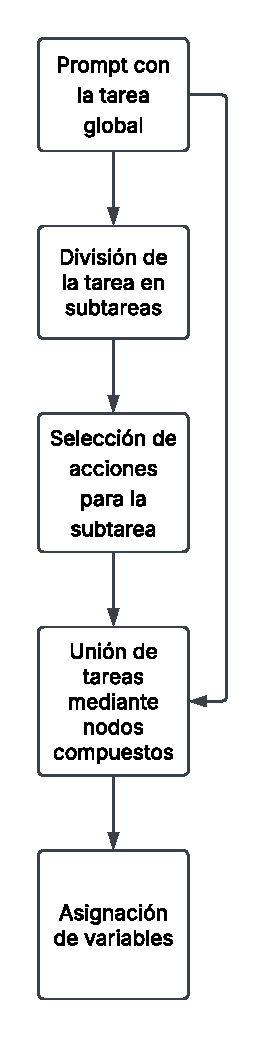
\includegraphics[width=0.2\textwidth]{Imagenes/Vectorial/GeneracionSubtareas.pdf}
    \caption[Generación mediante subtareas]{Diagrama de flujo de la generación de \glspl{BT} mediante división en subtareas}
    \label{fig:generacionSubtareas}
\end{figure}

Finalmente se descartó esta opción debido a que los árboles resultantes quedaban muy planos (con menos niveles de profundidad de lo que se cabía esperar), hacieéndolos difícilmente legibles y modificables.
Además los agentes tendían a equivocarse (mala división en subtareas, confusión entre el tipo que debería ser un nodo padre) o a alucinar (inventarse tareas o decoradores que no existen), no consiguiendo de este modo un \gls{BT} válido con ninguno de los modelos probados.

Trabajos como \cite{SayCan} o \cite{LLMPlanner} muestran que, dado un conjunto de acciones posibles a realizar, los \glspl{LLM} son capaces de seleccionar de éstas un órden para realizar una tarea de alto nivel.
Es por ésto que se decidió que el \gls{LLM} generase esta secuencia en un formato de pseudocódigo que fuese fácilmente convertible al formato JSON deseado.
Este pseudocódigo se especifica de la siguiente manera:
\begin{itemize}
    \item Las palabras reservadas son: SEQUENCE, SELECTOR, PARALLEL, IF, THEN, ELSE, DO, END.
    \item Los bloques de nodos compuestos (como SELECTOR) deben acabar con la palabra END.
    \item Las condiciones deberán ser escritas como ``IF (nombre del condicional de la lista de decoradores) THEN''.
    \item Los condicionales serán usados por el nodo siguiente.
    \item Las acciones deberán ser escritas como ``DO (nombre de la acción de la lista de acciones)''. 
\end{itemize}

Se puede ver un ejemplo de este pseudocódgo en la figura \ref{fig:examplePseudocode}.

\begin{figure}[htbp]
  \begin{verbatim}
SELECTOR
    IF has_key THEN
        SEQUENCE
            DO move_to_door
            DO open_door
        END
    ELSE
        SEQUENCE
            DO find_key
            DO move_to_door
            DO open_door
        END
END
\end{verbatim}
  \caption{Ejemplo del pseudocódigo que el \gls{LLM} debe generar.}
  \label{fig:examplePseudocode}
\end{figure}

Como se ha podido ver en trabajos relacionados, la generación de \glspl{BT} mediante \glspl{LLM} mejora considerablemente en modelos a los que se le ha aplicado \gls{Fine-tuning} o se les proporciona ejemplos.
Debido a la falta de capacidad computacional no se ha podido hacer un \gls{Fine-tuning} de un \gls{LLM}, por lo que se ha optado a recopilar una pila de ejemplos de \glspl{BT} para poder hacer un sistema \gls{RAG}.
Para ello se ha escogido el dataset publicado por \cite{llmbrain}\footnote{Enlace a la página de Hugging Face: \url{https://huggingface.co/datasets/ArtemLykov/LLM_BRAIn_dataset}}, el cual contiene 8366 ejemplos de \glspl{BT}.
Debido a que estos \glspl{BT} están en formato XML no se pueden utilizar de forma predeterminada para el sistema RAG, por lo que se ha procedido a hacer un preprocesamiento de los datos.
Este proprocesado carga el dataset desde Hugging Face, los limpia y los traduce al formato necesario.
La limpieza consiste en el uso de expresiones regulares para poder subsanar los fallos de formato más comunes que tenían estos datos, como diferencias entre nombres por mayúsculas y minúsculas, etiquetas sin la apertura o la clausura, faltas de comillas, etc.
Si hay algún ejemplo que, aun con la limpieza, no se ha conseguido parsear por otro fallo, se descarta.
Finalmente, de los 8366 ejemplos se quedaron 8290 \glspl{BT} válidos.
Una vez los datos están limpios, se procede a la traducción del formato XML gracias al módulo ``xml.etree.ElementTree'' mediante una función recursiva que recorre el XML y va construyendo todo el árbol.
Cuando el árbol ha sido construído se guarda en formato JSON siguiendo el JSON Schema especificado para este trabajo, y finalmente se traduce al pseudocódigo especificado previamente gracias a otra función recursiva, quedando así 8366 archivos JSON con el prompt de la acción de alto nivel a realizar, el \gls{BT} resultante y el pseudocódigo.

Con los ejemplos de \glspl{BT} preparados se ha procedido a la aplicación del sistema \gls{RAG}.
Al iniciar la herramienta de generación se crea el \gls{Almacén vectorial} cargando los documentos mencionados anteriormente en estructuras llamadas ``Document'', provenientes del módulo ``langchain\_core.documents''.
Una vez están todos los documentos cargados se procede a hacer el \gls{Embedding} de éstos de manera local gracias al modelo de Hugging Face ``all-MiniLM-L6-v2'' mediante el módulo ``langchain\_huggingface''.
Estos \glspl{Embedding} se crean y se almacenan en una estructura de tipo \gls{FAISS} gracias al módulo ``langchain\_community.vectorstores''.
Una vez creado el \gls{Almacén vectorial} se rescatan las 5 búsquedas más similares al comportamiento pedido por el usuario y se incluyen en el prompt del sistema del \gls{LLM}.

Para la generación de pseudocódgo a partir del comportamiento buscado se ha requerido un modelo de mayor tamaño que los previamente usados, por lo que se ha usado el \gls{LLM} ``Mistral Large 3'', el cual cuenta con un total de 41B de parámetros, mediante el módulo ``langchain\_mistralai'', el cual realiza llamadas de \gls{api} al modelo.
Para el prompt de sistema del modelo se han realizado varias técnicas de \textit{prompt engineering} con el fin de reducir las alucinaciones en la generación del pseudocódgo:

\begin{itemize}
    \item \texttt{Role prompting}: Se le especifica al \gls{LLM} como debe actuar: ``You are an expert in behavior trees and algorithm design.''.
    \item \texttt{Especificación de la tarea}: Se le especifica para qué tarea debe responder: ``Your task is to convert a high-level task description into a structured pseudocode algorithm that can later be transformed into a Behavior Tree.''.
    \item \texttt{Few-shot prompting}: Se le especifican varios ejemplos, sacados del sistema \gls{RAG} mencionado anteriormente.
    \item \texttt{Chain-of-Thought}: Obliga al modelo a, internamente, seguir la línea de pensamiento representada en la figura \ref{fig:CoT-Code}
    \item \texttt{Self‑Critique Prompting}: Le pide al modelo que evalúe su respuesta buscando si se ha inventado acciones o condicionales. Esto se hace en una segunda llamada con el siguiente prompt: ``Verify if your pseudocode is made only with the actions and conditions available. Responde me with ONLY the final pseudocode and no explanations or plain text''
\end{itemize}

\begin{figure}[H]
    \centering
    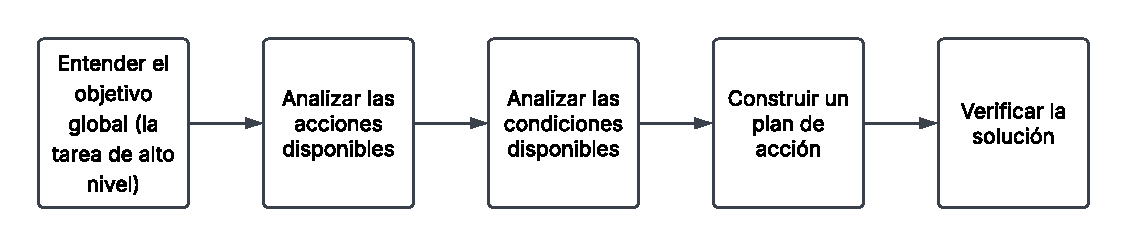
\includegraphics[width=1\textwidth]{Imagenes/Vectorial/CoT-TFM.pdf}
    \caption[Chain-of-Thought del \gls{LLM} que genera el pseudocódgo.]{Diagrama de la cadena de pensamiento que sigue el \gls{LLM} generador de pseudocódigo.}
    \label{fig:CoT-Code}
\end{figure}

El prompt de sistema completo se puede ver en el apéndice \ref{appendix:spCode}.

Una vez se ha generado el pseudocódigo se procede a la traducción de éste al formato JSON.
Esto se hace mediante la clase ``BehaviorTreeParser'' y mediante dos clases auxiliares: Composite y Action, las cuales ambas heredan de la clase Node.
La clase Composite contiene el tipo (un string), una lista de nodos hijos (lista de tipo ``Node''), un decorador (opcional de tipo string), las variables de la \gls{BB} del decorador (una lista de strings) y un identificador (un entero).
La clase Action tiene el nombre de la tarea (un string), las variables de la \gls{BB} que puede usar la tarea (una lista de strings), un decorador (opcional de tipo string), las variables de la \gls{BB} del decorador (una lista de strings) y un identificador (un entero).
Para la traducción del pseudocódigo primero se preprocesa guardando cada línea en una lista de strings.
Seguido de esto se procesa cada línea dividiendo cada palabra de ésta y actuando dependiendo de cuál es su primera palabra:
\begin{itemize}
    \item \texttt{SEQUENCE, SELECTOR o PARALLEL}: Se crea un nodo de tipo ``Composite'', se establece su tipo como la palabra usada y se verifica si hay una condición pendiente. Si es el caso, se establece esta condición. Además, se añade este nodo a su padre (en el caso de haberlo es el último nodo añadido a una pila auxiliar) y se añade a la pila auxiliar.
    \item \texttt{IF}: Se verifica si tiene un condicional o si el condicional que tiene existe. En caso contrario de cualquiera de los dos se lanza un ``ParserError'' indicando la línea y el fallo. En el caso de que no haya error se establece la condición como la condición pendiente.
    \item \texttt{DO}: Se verifica si tiene una acción o si esa acción existe. Al igual que en el caso anterior, de no ser así se lanza un ``ParserError''. En caso de haberlo se crea un nodo de tipo ``Action'' con el nombre de la acción que hay a continuación. Igualmente que con los nodos compuestos, se verifica si hay alguna condición pendiente y se añade el nodo al padre.
    \item \texttt{END}: Se verifica que la pila no esté vacía. En caso contrario significa que hay un ``END'' sin bloque que cierre, por lo que se lanza un ``ParserError''. En caso de que sí esté vacía se saca un nodo de la pila. A continuación se verifica si la pila se ha quedado vacía, lo que significaría que ese nodo era la raíz del árbol. En caso de ya haber raíz se lanza un ``ParserError'' indicando que hay múltiples raíces.
\end{itemize}
Una vez se acaba este procesamiento de cada línea se verifica si sigue habiendo pila (lo que indicaría que hay bloques sin cerrar) o si no se ha generado una raíz.
Los posibles ``ParserError'' lanzados durante este proceso se recogen fuera de esta función para poder volver llamar al \gls{LLM} indicando el error de la excepción con el fin de que devuelva un pseudocódigo arreglado.

Cuando ya ha sido procesado todo el pseudocódigo se crea una clase auxiliar llamada ``BlackboardAssignmentAgent'' que se encarga de asignar las variables de la \gls{BB} a las tareas o los decoradores.
Para ello reconstruye el pseudocódigo asignándole el identificador a cada nodo (este identificador es el órden de aparición de cada acción o decorador, ya que en los \glspl{BT} es normal que se repitan) y se le pide a un segundo \gls{LLM} que a cada decorador y acción que necesite una variable de la \gls{BB} se le asigne.
Por problemas con sobrecarga de peticiones de la \gls{api}, para este caso se usa un modelo local más pequeño, el modelo ``llama3:8b''.
Para el prompt de sistema de este \gls{LLM} se le pasa el árbol en el formato del pseudocódigo reconstruido mencionado anteriormente, la lista de las acciones que necesitan una variable de la \gls{BB} con sus descripciones y la lista de variables de la \gls{BB}.
Para disminuir las alucinaciones de este \gls{LLM} se han usado las siguientes técnicas de \textit{prompt engineering}:

\begin{itemize}
    \item \texttt{Role prompting}: ``You are an expert in Unreal Engine Behavior Trees.''
    \item \texttt{Especificación de la tarea}: ``Your task is NOT to understand the whole game. Your ONLY task is assigning Blackboard variables to Behavior Tree nodes.''
    \item \texttt{One-shot prompting}: Se le especifica un ejemplo inventado mostrado en la figura \ref{fig:examplePseudocodeBB}
\end{itemize}

\begin{figure}[htbp]
  \begin{verbatim}
Example Input:
Actions : grab_key : Stores the key in the inventory,
    move_to : Moves to a position,
    open_door: Open a door
Variables: ["Key" : "Object", "Door" : "Object", "Enemy_position" : "Vector3"]
Tree:
SEQUENCE
    DO move_to#1
    DO grab_key#1
    DO move_to#2
    DO open_door#1 [Decorator=IsNear?#1]
    DO wave#1

Output format: 
{
    "Actions": {
        "move_to#1":["Key"],
        "grab_key#1":["Key"],
        "move_to#2":["Door"],
        "open_door#1":["Door"]
    },

    "Decorators": {
        "IsNear?#1":["Door"]
    }
}
\end{verbatim}
  \caption{Ejemplo del input y el output del \gls{LLM} que establece las variables de la \gls{BB}.}
  \label{fig:examplePseudocodeBB}
\end{figure}

Una vez genera la respuesta se valida el resultado comprobando si todos los nombres (variables y acciones) son correctos.
Cuando el resultado es válido se guardan las variables asignadas en los nodos correspondientes y, finalmente, se construye el JSON mediante una función recursiva desde la raiz del árbol y se guarda en un archivo con el nombre especificado por el usuario.

Trabajos como \cite{PlanBench} han demostrado que la planificación generada por \glspl{LLM} como se ha hecho en este trabajo no resultan ser fiables de forma exacta, por lo que se ha diseñado un sistema de validación y corrección de errores automático.